\section{Use case model}

\begin{figure}[H]
	\centering
	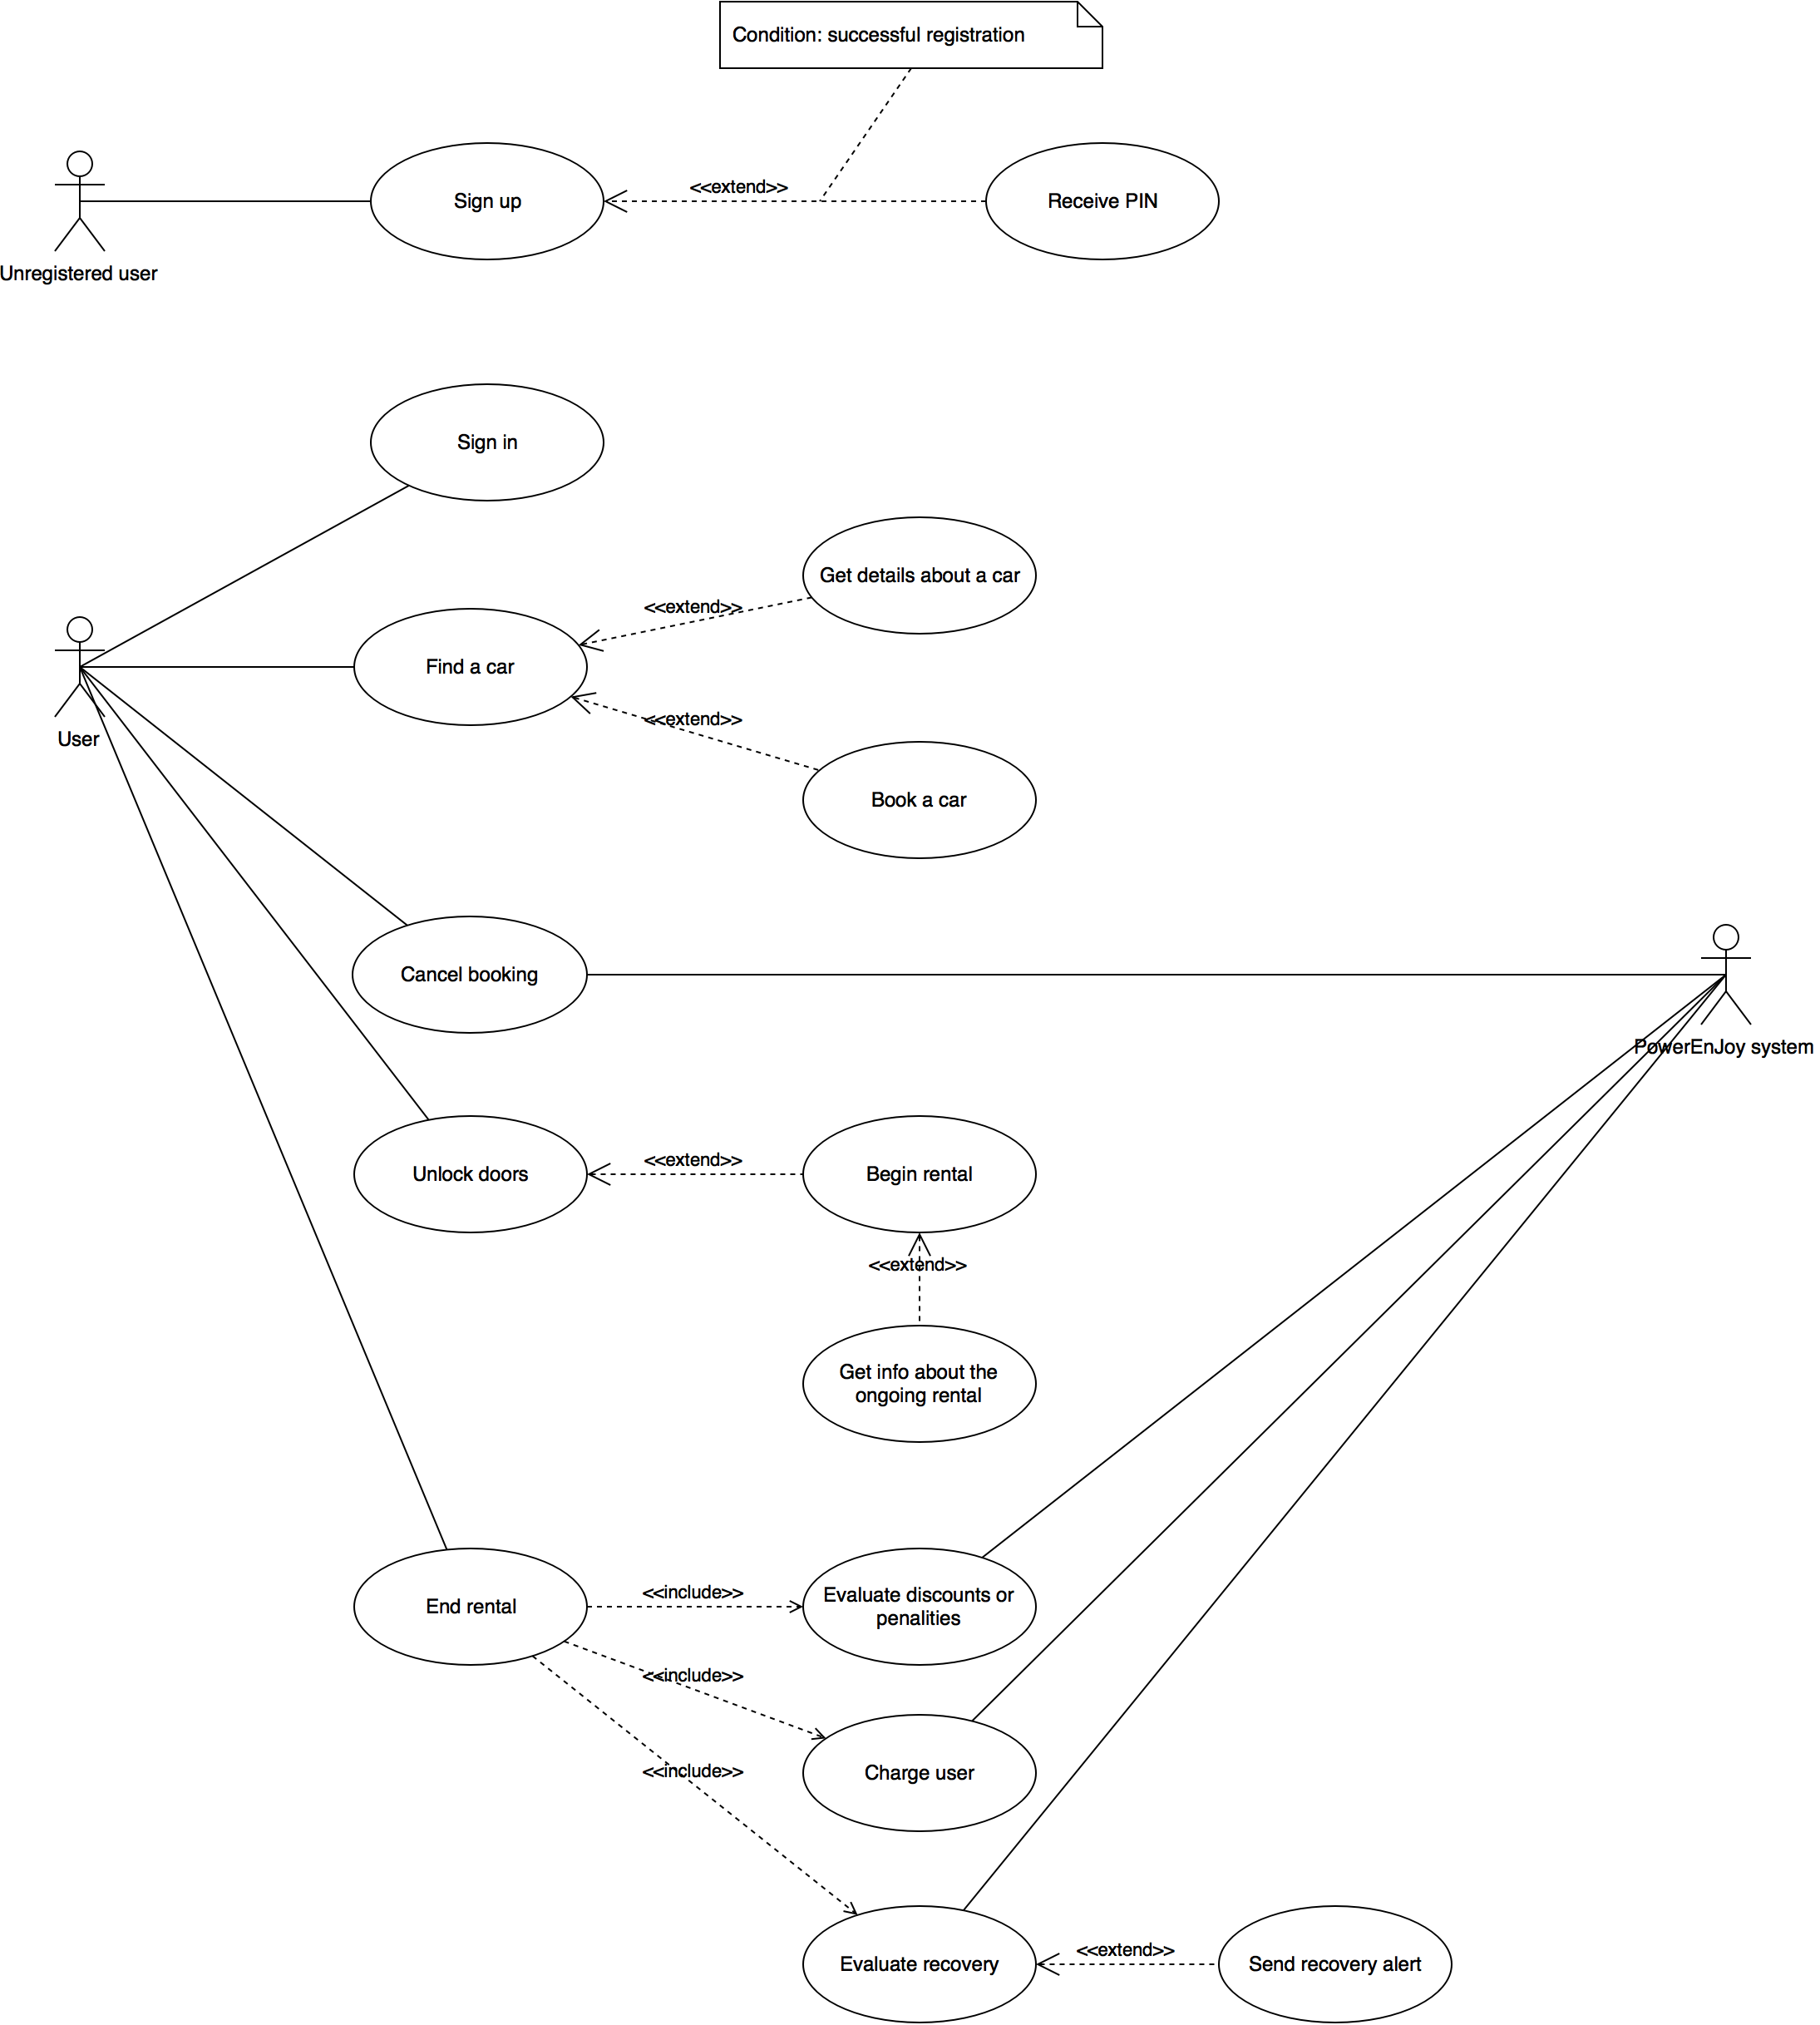
\includegraphics[width=\textwidth]{use-case-model}
	\caption[Use case model]{The diagram above represents the use case model of the PowerEnJoy project. The actors included are the unregistered user, the user and the PowerEnJoy system.}
	\label{fig:use-case-model}
\end{figure}

\subsection{Use case description 1 - Sign up}
\begin{labeling}{use-case-desc-1}
		\item[\textbf{Name}] Sign up
		\item[\textbf{Actors}] User
		\item[\textbf{Entry conditions}] There are no entry conditions.
		\item[\textbf{Flow of events}]
			\begin{itemize}
				\item[]
				\item The user accesses the homepage of PowerEnJoy or opens the app.
				\item The user inserts his/her credentials in the registration form.
				\item The user clicks on the sign up button.
				\item The system processes the registration of the user.
			\end{itemize}
		\item[\textbf{Exit conditions}] The user is successfully registered to the system.
		\item[\textbf{Exceptions}]
			\begin{itemize}
				\item[]
				\item Credentials provided by the user are not correct. In this case the system notifies the user of the error and let him/her to input again his/her credentials. 
				\item User is already registered. In this case the system notifies the user of the impossibility to register.
			\end{itemize}
	\end{labeling}

\subsection{Use case description 2}
\subsection{Use case description 3}